\documentclass{article}
\usepackage[utf8]{inputenc}
%%\documentclass{article}
\usepackage{movie15}
\usepackage{graphicx}
\usepackage{amsmath}
\usepackage{amssymb}
\usepackage{float}
\title{security_ARP Attack design}
%%\author{ }
\date{July 2019}


\vspace{1cm}
\hspace{5cm}
 
 \begin{center}
    \huge
    \textbf{ARP Cache Poisoning } 
 \end{center}
 
 
\begin{figure}[h]
    \centering

\includegraphics[width=0.2\textwidth]{images/buet_logo_1.png}
\end{figure}
 
 



\begin{center}
    \\
 Prepared By\\
MD.Omer Danish\\ \\
Student ID: 1505053
\\
Group No : 01\\
Section : A\\


\end{center}


\begin{center}
Submitted to \\
Dr. Md. Shohrab Hossain\\
Associate Professor\\ \\

\Large
Department of Computer Science \\ \\
Bangladesh University of Engineering and Technology\\ \\ \\
\linebreak

\end{center}


\date{\today}

\newpage
\begin{document}
\tableofcontents
\newpage
%%\maketitle
%%\section{Brief of Our ARP Cache Poisoning}


\section{Why do I think it was successful}
\textbf{ARP Cache Poisoning} is a technique by which an attacker sends (spoofed) Address Resolution Protocol (ARP) messages onto a local area network. Generally, the aim is to associate the attacker's MAC address with the IP address of another host, such as the default gateway, causing any traffic meant for that IP address to be sent to the attacker instead.

\textbf{ARP Cache Poisoning} can create many unusual behavior in  network. Some of them are 
\renewcommand\labelitemi{$\square$}
\begin{itemize}
    \item  Denial of service
    \item  Man in the middle 
    \item Stop all traffic
    \item  Session hijacking
    
\end{itemize}
The reason why our attack is successful are 


\begin{itemize}
    \item  Our attack is successful because after performing our ARP Cache Poisoning Attack it has changed the victim's ARP table.In the victim's ARP table for both attacker and gateway there is a single MAC address.That means any packet from victim to gateway will not be delivered to only gateway but also to the attacker.

    \item  Our attack has stopped the packet transfer between gateway and victim.That means victim is unable to access internet.Thus Denial of Service is performed through ARP cache poisoning.

\end{itemize}

\section{Steps of Attack}
There are mainly two steps .At first step our attack will poison victim's ARP Cache. In the second step our attack will restrict victim from using internet. Let's see each step individually.

\subsection{MAC table changing part}

\begin{figure}[H]
\centering
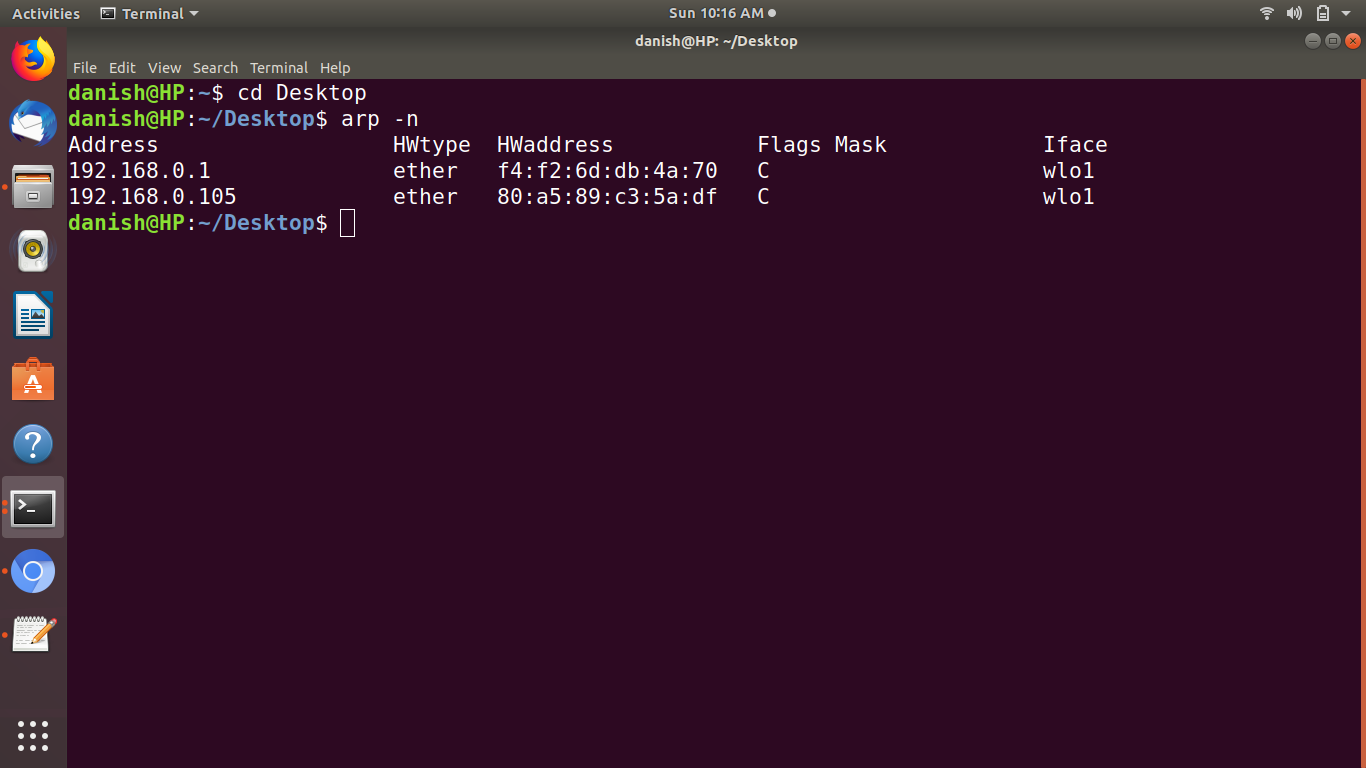
\includegraphics[width=\textwidth]{images/attacker_pc_before_cache_table_attack.png}
\caption{\texttt{ attacker\_pc\_before\_cache\_table\_attack}}
\end{figure}

\begin{figure}[H]
\centering
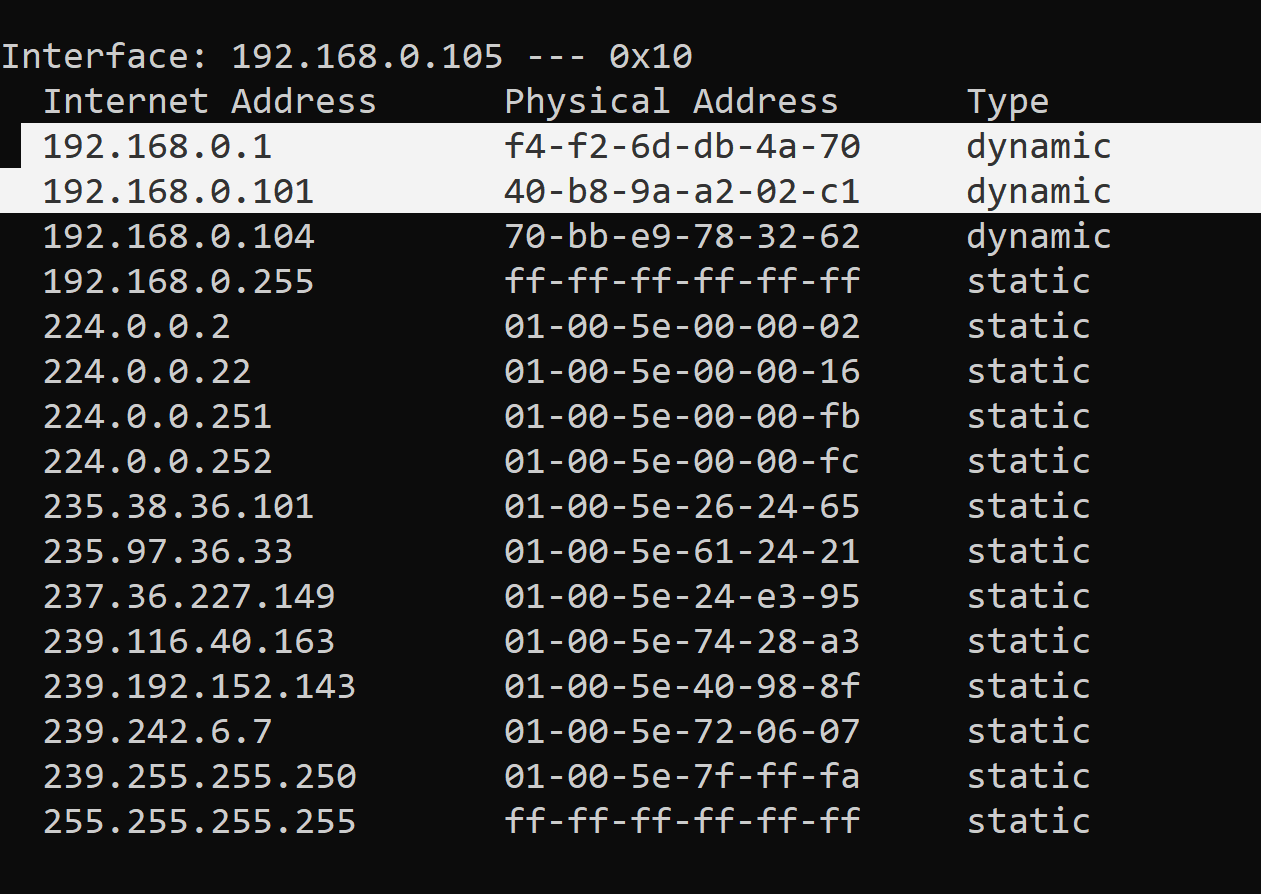
\includegraphics[width=\textwidth]{images/victim_pc_before_cache_table_attack.png}
\caption{\texttt{victim\_pc\_before\_cache\_table\_attack}}
\end{figure}
\textbf{How to run}
\newline
General Command ::sudo python ./cachetablepoisoner.py -g   gateway-ip -t   target-ip

Example Command ::sudo python ./cachetablepoisoner.py -g 192.168.0.1 -t 192.168.1.105
\begin{figure}[H]
\centering
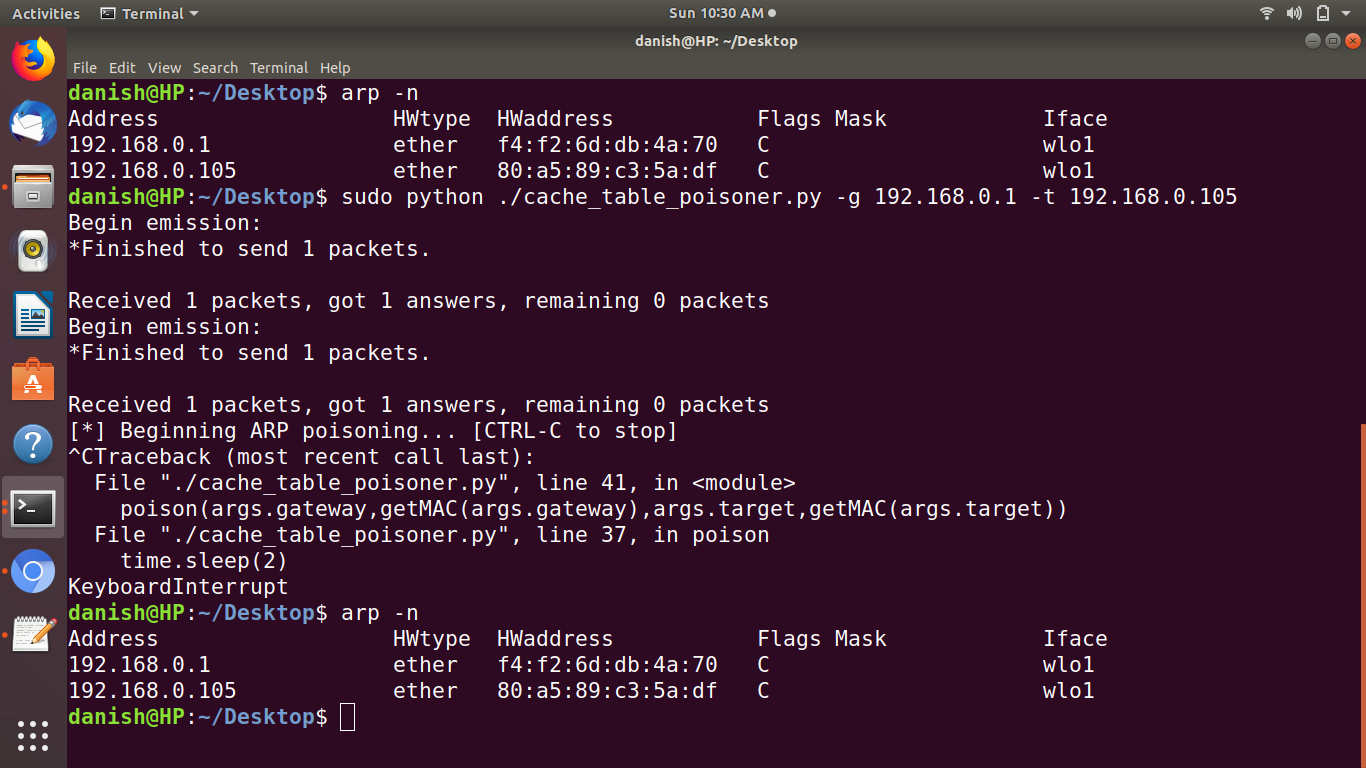
\includegraphics[width=\textwidth]{images/attacker_pc_after_cache_table_attack.png}
\caption{\texttt{attacker\_pc\_after\_cache\_table\_attack}}
\end{figure}

\begin{figure}[H]
\centering
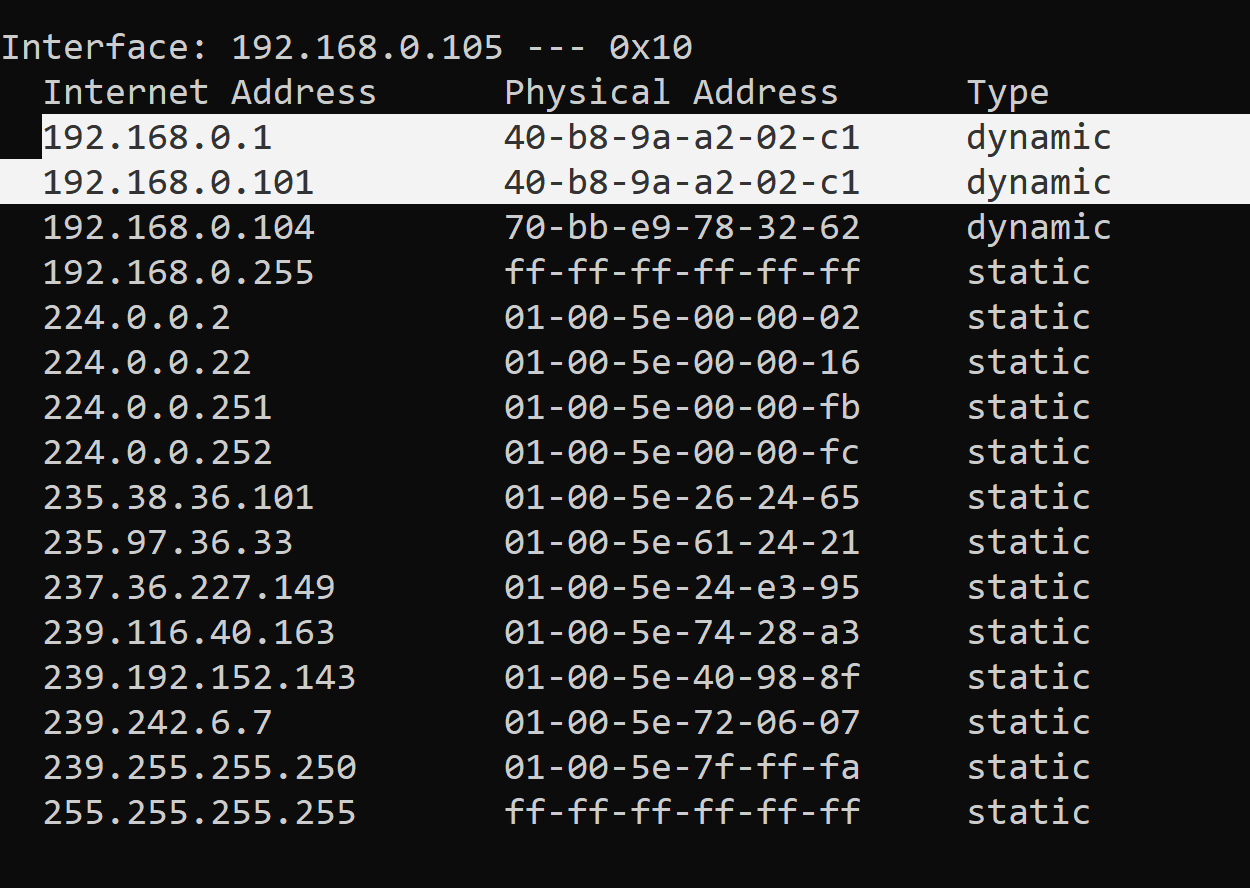
\includegraphics[width=\textwidth]{images/victim_pc_after_cache_table_attack.png}
\caption{\texttt{victim\_pc\_after\_cache\_table\_attack}}
\end{figure}


\subsection{Denial of service part}
\textbf{How to run}
\newline
General Command :
\texttt{sudo python2 denial\_of\_service\_arpspoof.py $-i$ interface $-t$ target\_1\_IP,target\_2\_IP,target\_3\_IP $-g$ Default\_\Gateway(Router$_$IP)}
Example Command 	:
\texttt{sudo python2 denial\_of\_service\_arpspoof.py $-i$ wlo1 $-t$ 192.168.0.105 $-g$ 192.168.0.1}
\begin{figure}[H]
\centering
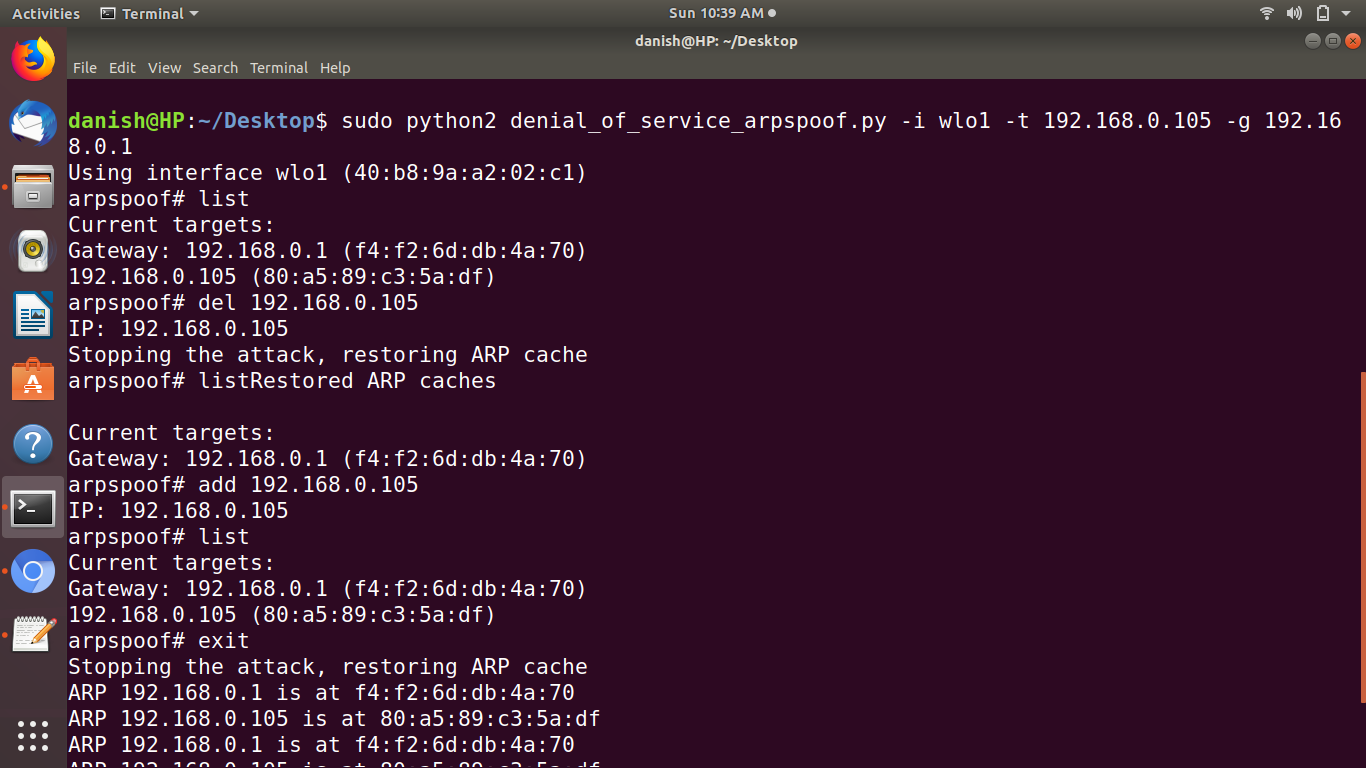
\includegraphics[width=\textwidth]{images/attacker_pc_after_denial_1_attack.png}
\caption{\texttt{attacker\_pc\_after\_denial\_1\_attack  }}
\end{figure}
\begin{figure}[H]
\centering
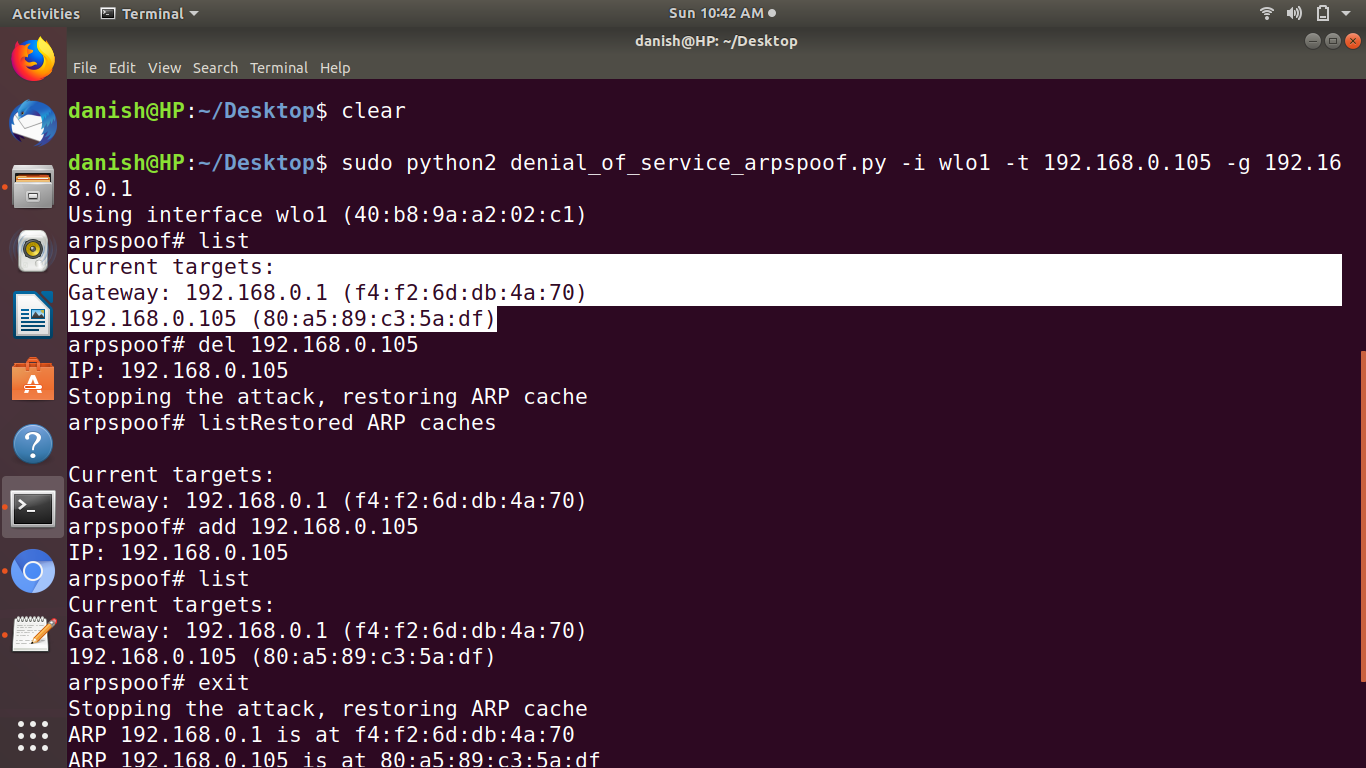
\includegraphics[width=\textwidth]{images/attacker_pc_after_denial_2_attack.png}
\caption{\texttt{ attacker\_pc\_after\_denial\_2\_attack}}
\end{figure}
\section{Counter measure of ARP Cache Poisoning}
Counter measures are divided into two types.First is preventing measures and second is detecting measures.
The simplest form of certification is the use of static, read-only entries for critical services in the ARP cache of a host. IP address-to-MAC address mappings in the local ARP cache may be statically entered. Hosts don't need to transmit ARP requests where such entries exist. While static entries provide some security against spoofing, they result in maintenance efforts as address mappings for all systems in the network must be generated and distributed. This does not scale on a large network since the mapping has to be set for each pair of machines resulting in n2-n ARP entries that have to be configured when n machines are present; On each machine there must be an ARP entry for every other machine on the network; n-1 ARP entries on each of the n machines.
\end{document}
